\subsection{Deep Laplacian Pyramid Network (LapSRN\cite{LapSRN}) and Multi-scale Deep Laplacian Pyramid Network (MS-LapSRN \cite{MSLapSRN})}\label{lapsrn}

\subsubsection{Features}
\textbf{LapSRN} in order to be able to reconstruct the SR image uses:
\begin{itemize}
    \item \textbf{Charbonnier loss} because the L2 loss is not able to capture the underlying mapping of LR images to many HR images.
    \item \textbf{progressive reconstruction} of the SR image using the Laplacian Pyramid 
    Framework \cite{laplacianpyramid}.
    \item \textbf{residual learning}: learn the summation between the laplacian extracted by \textit{features extraction branch} and the upscaled LR image in the \textit{image reconstruction branch}
\end{itemize}
\textbf{MS-LapSRN} improve LapSRN introducing:
\begin{itemize}
    \item \textbf{parameter sharing} across pyramid level and within pyramid levels in order to reduce the amount of parameters which increase with the scale (the greater the scale the deeper the network since there are more levels).
    \item \textbf{local skip connections} for avoiding the vanishing/exploding gradient prolem with the increase in the depth of the network.
    \item \textbf{multi scale training}: the previous network was trained for each scale different networks.
\end{itemize}

\subsubsection{Architecture}
\begin{figure}
    \centering
    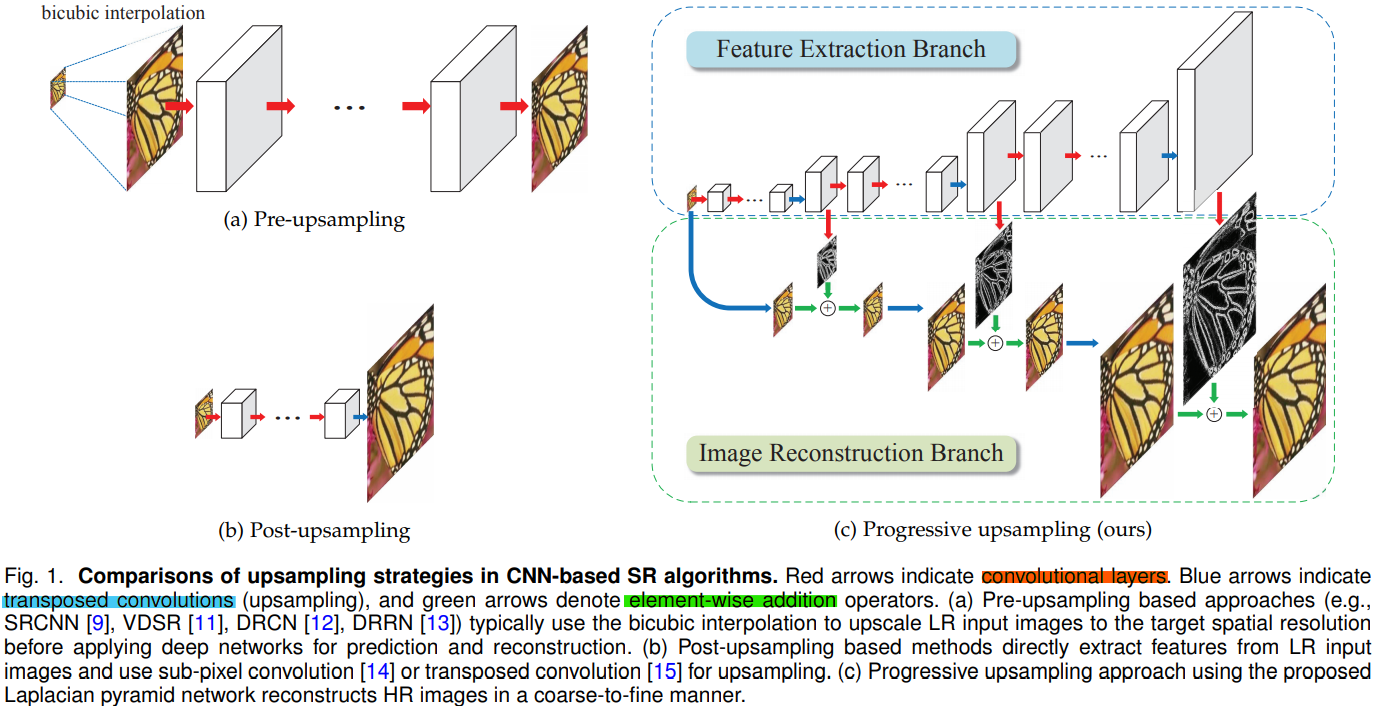
\includegraphics[width=\textwidth, keepaspectratio]{lapsr-old-model.png}
    \caption{LapSRN architecture.}\label{lapsrn:old}
\end{figure}

\begin{figure}
    \centering
    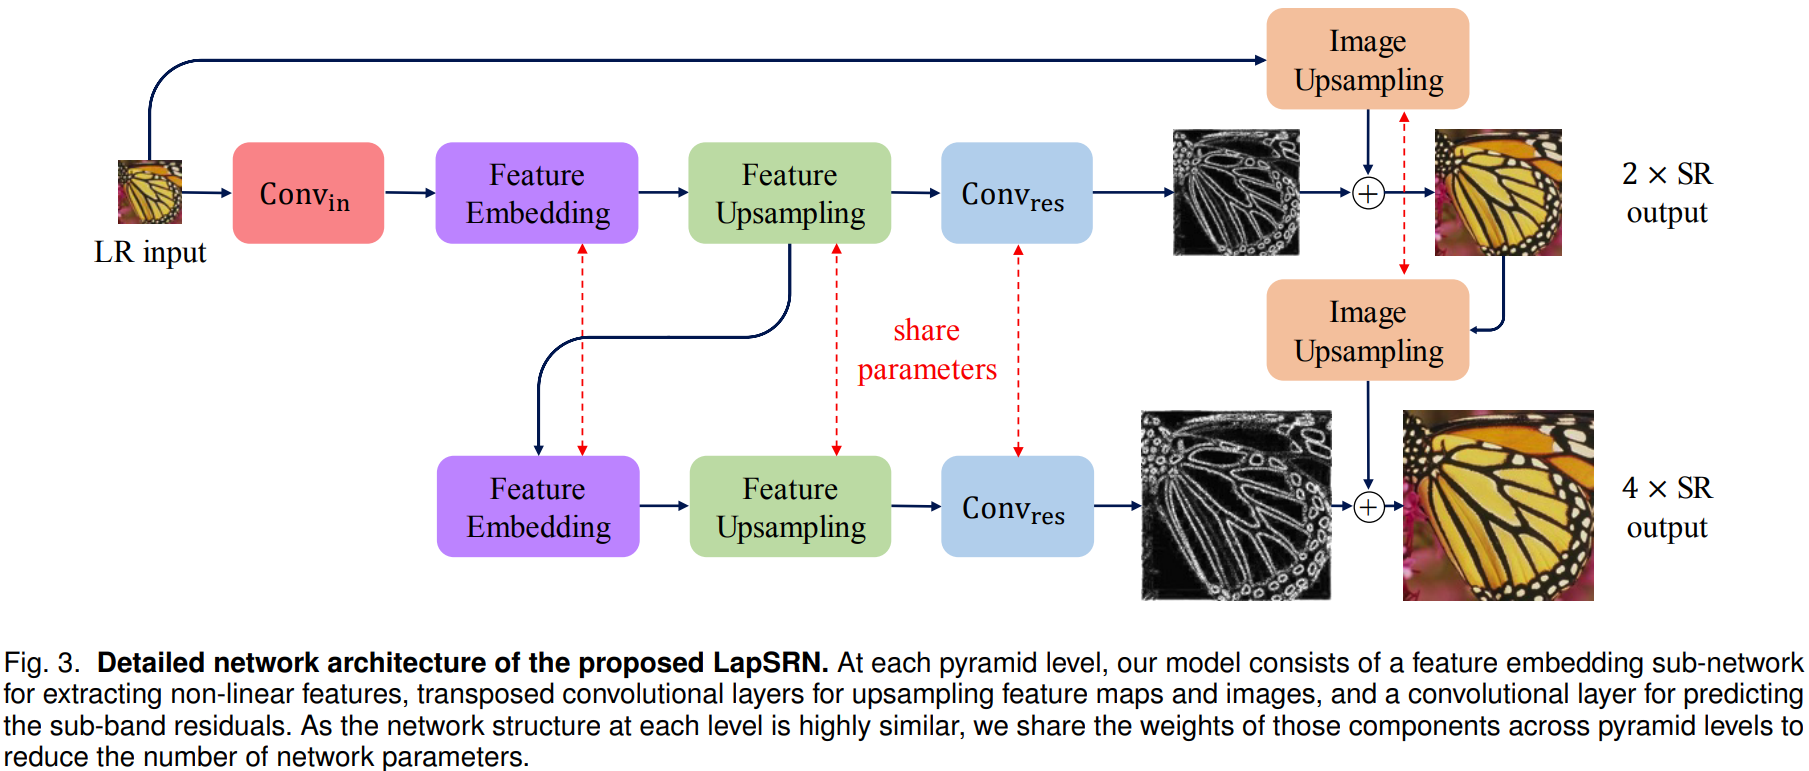
\includegraphics[width=\textwidth, keepaspectratio]{lapsr-new-model.png}
    \caption{MS-LapSRN architecture.}\label{lapsrn:new}
\end{figure}
In \textit{LapSRN} [\Cref{lapsrn:old}] the \textbf{feature extraction branch} extract laplacian representations which are used for training (in an end-to-end fashion) the \textbf{image reconstruction branch} in order to reconstruct the SR image at the last level (due to the laplacian pyramid framework training on an higher scales lead to have also a network capable to resolve SR task for lower scale).

The residual learning allow the network to focus on high-frequency information (edges) instead of low-frequency ones.

In the \textit{MS-LapSRN} [\Cref{lapsrn:new}] the feature extractor ($Conv_{in}$, Feature Embedding, Feature Upsampling, $Conv_{res}$) has always the same function: extract meaningful information from an input image in order to create a residual whose spatial dimension in 2x then the input one; therefore is logic to use same weights for doing so.

The \textit{Feature embedding} has \textbf{R} recursive block \cite{DRCN} \cite{DRRN} which contains distinct \textbf{D} convolutional layers.

\begin{figure}
    \begin{subfigure}{0.49\textwidth}
        \centering
        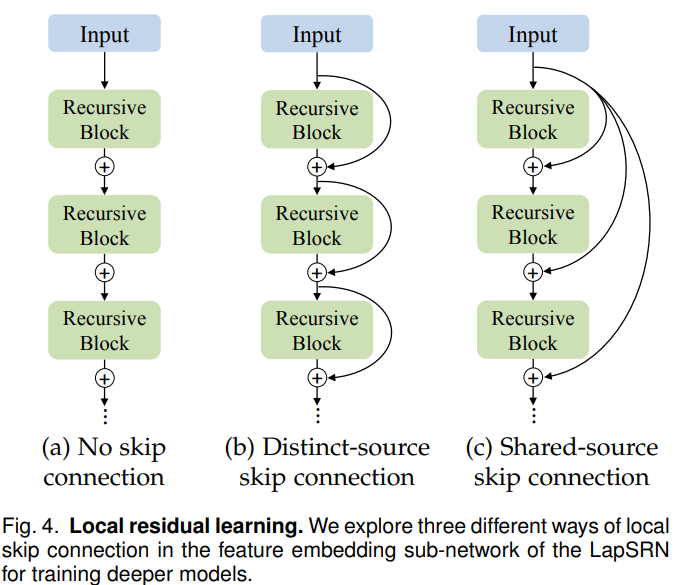
\includegraphics[width=\textwidth, keepaspectratio]{lapsr-recursive-block-differences.png}
        \caption{Differences between local skip connections.}            
    \end{subfigure}
    \begin{subfigure}{0.49\textwidth}
        \centering
        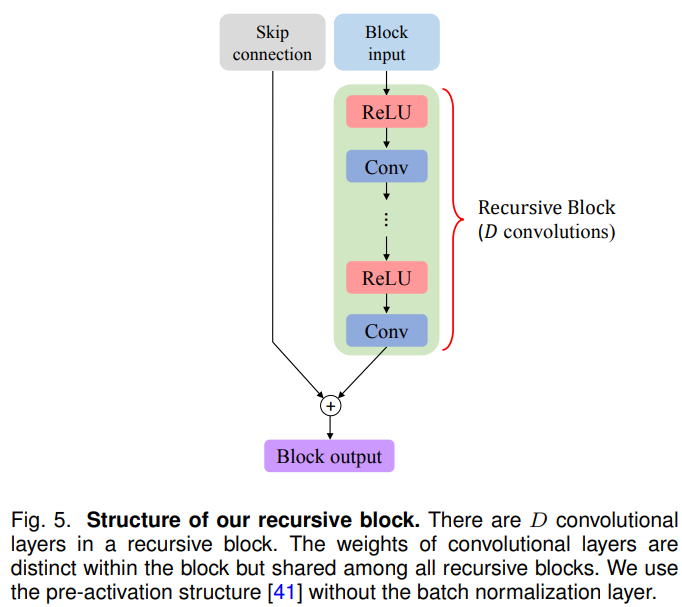
\includegraphics[width=\textwidth, keepaspectratio]{lapsr-recursive-block.png}
        \caption{Recursive block used in MS-LapSRN.} \label{lapsrn:recursiveblock}
    \end{subfigure}
\end{figure}

The structure of the recursive block [\Cref{lapsrn:recursiveblock}] use a skip connection directly connected to the input and a pre-activation inside the residual path \cite{resnetidentity}.

Recursive block (or single convolution) allow to reduce the number of parameters and increase the depth of the network as well as the receptive field of the network in the last activation without increasing the memory footprint of the network. 

\subsubsection{Loss}
Both \textit{LapSRN} and \textit{MS-LapSRN} use the \textbf{Charbonnier loss}: the former use it once the latter at each level; the equation is the following:
$$
L_S = \frac{1}{N} \sum_{i=1}^{N}\sum_{l=1}^{L} \rho \times \left( \left( y_l^{(i)}-x_l^{(i)} \right) - r_l^{(i)} \right)
$$ where $S$ is the target upsampling factor, $\rho = \sqrt{x^2+\epsilon^2}$ (Charbonnier penalty function which is a differentiable L1 norm), $x_l$ is the upscaled LR image at level l, $y_l$ is the downscaled HR target image (y) at level l and $r_l$ is the residual at level l.

The final loss is the sum of the loss for each level trained using images with different scales (\textbf{multi scales training}):
$$
L= \sum_{s \in [2,4,8]} L_s
$$
\subsubsection{Depth}
The depth of the network is: $ (D \times R + 1) \times (L + 2)$ where $D$ is the number of convolutions inside each recursive block, $R$ is the number of recursive blocks, $+1$ represents the transposed convolution, $+2$ represent the convolutions that perform feature extraction and residual hallucination.
\subsubsection{Results}

Here will be presented only the results of \textbf{MS-LapSRN}\cite{MSLapSRN} since it's an evolution of LapSRN.

\paragraph{Ablation studies on pyramid structure, global residual learning and loss}
\begin{figure}
    \begin{subfigure}{0.49\textwidth}
        \centering
        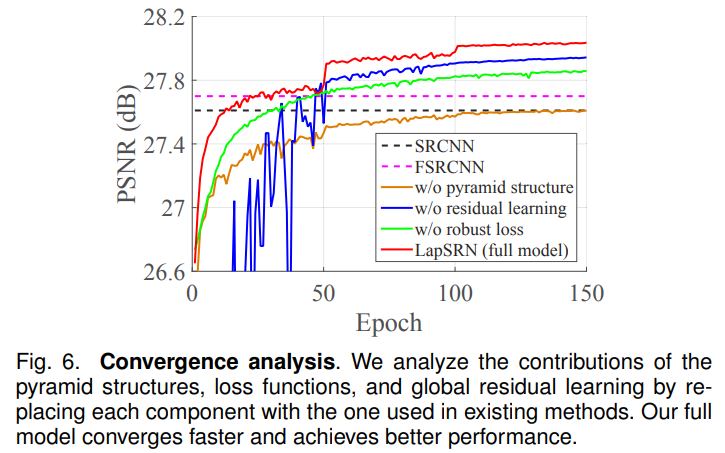
\includegraphics[width=\textwidth, keepaspectratio]{lapsr-convergence-analysis.png}
        \caption{Study on performance with different settings.}
    \end{subfigure}
    \begin{subfigure}{0.49\textwidth}
        \centering
        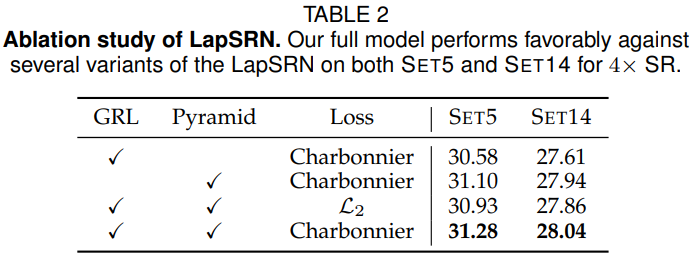
\includegraphics[width=\textwidth, keepaspectratio]{lapsr-ablation-studies.png}
        \caption{Ablation study on LapSRN.}
    \end{subfigure}
    \begin{subfigure}{0.49\textwidth}
        \centering
        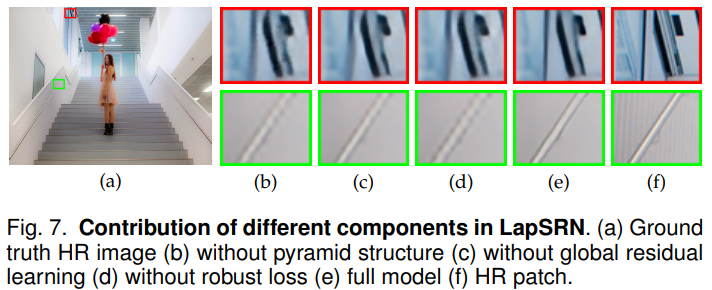
\includegraphics[width=\textwidth, keepaspectratio]{lapsr-contribution-studies.png}
        \caption{Contribution of different components in LapSRN.}
    \end{subfigure}
    \begin{subfigure}{0.49\textwidth}
        \centering
        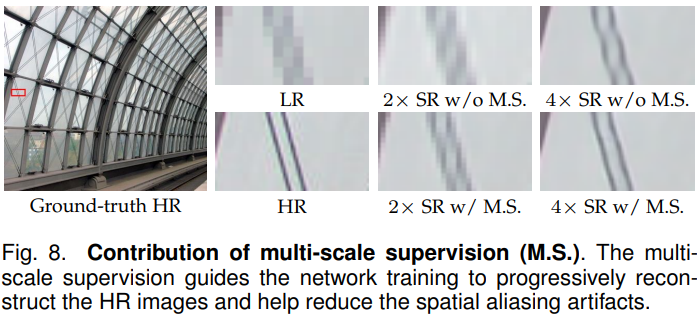
\includegraphics[width=\textwidth, keepaspectratio]{lapsr-multiscale-studies.png}
        \caption{Contribution of multi-scale supervision.}
    \end{subfigure}
    \caption{Performance studies done on MS-LapSRN}\label{lapsr:performance-studies}
\end{figure}

From the performance studies [\Cref{lapsr:performance-studies}] it's possible to observe the contribution of each component used for the final result: the pyramid structures allow a faster convergence, the Charbonnier loss a better performance, the global residual learning both.

\paragraph{Studies on local skip connections}
\begin{figure}
    \begin{subfigure}{0.49\textwidth}
        \centering
        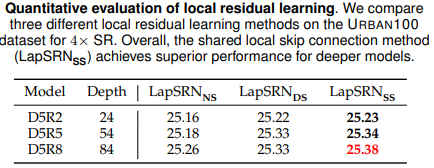
\includegraphics[width=\textwidth, keepaspectratio]{lapsr-local-skip-connection-studies.png}
    \end{subfigure}
    \begin{subfigure}{0.49\textwidth}
        \centering
        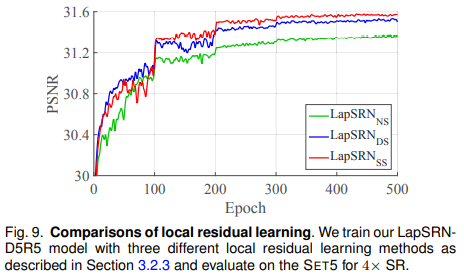
\includegraphics[width=\textwidth, keepaspectratio]{lapsr-local-skip-connection-graph.png}
    \end{subfigure}
    \caption{Local skip connection studies done on MS-LapSRN}\label{lapsr:lsc-studies}
\end{figure}
From the local skip connection studies [\Cref{lapsr:lsc-studies}] we can se that the best is \textit{shared source} (\textbf{SS}) which use as identity the same input.

\paragraph{Studies on parameter sharing}
\begin{figure}
    \begin{subfigure}{0.49\textwidth}
        \centering
        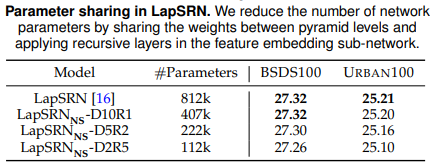
\includegraphics[width=\textwidth, keepaspectratio]{lapsr-paramters-studies.png}
    \end{subfigure}
    \begin{subfigure}{0.49\textwidth}
        \centering
        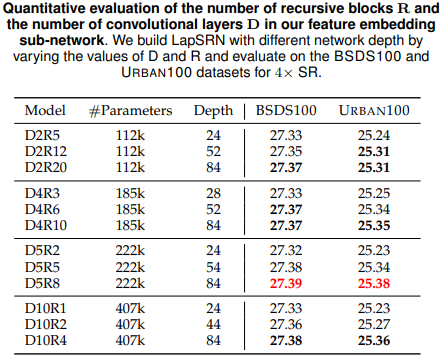
\includegraphics[width=\textwidth, keepaspectratio]{lapsr-parameters-studies.png}
    \end{subfigure}
    \begin{subfigure}{0.49\textwidth}
        \centering
        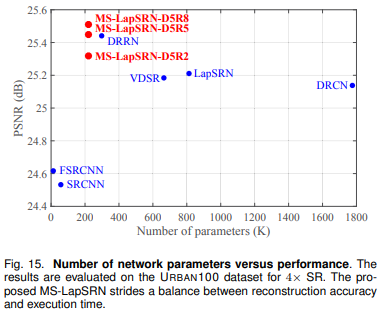
\includegraphics[width=\textwidth, keepaspectratio]{lapsr-parameters-performance.png}
    \end{subfigure}
    \begin{subfigure}{0.49\textwidth}
        \centering
        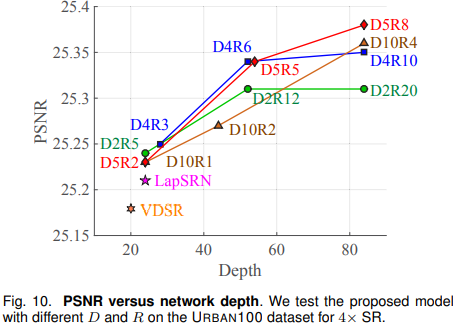
\includegraphics[width=\textwidth, keepaspectratio]{lapsr-depth-studies.png}
    \end{subfigure}
    \caption{Studies on parameters (weights) and hyperparameters D and R on MS-LapSRN}\label{lapsr:parameters-studies}
\end{figure}
From the parameters studies [\Cref{lapsr:parameters-studies}] it's possible to see the effectiveness of using recursive block which allow to have a deeper network with an increase of performance without too much parameters and also a faster inference time.

\paragraph{Quantitative and qualitative results}

\begin{figure}
    \begin{subfigure}{0.49\textwidth}
        \centering
        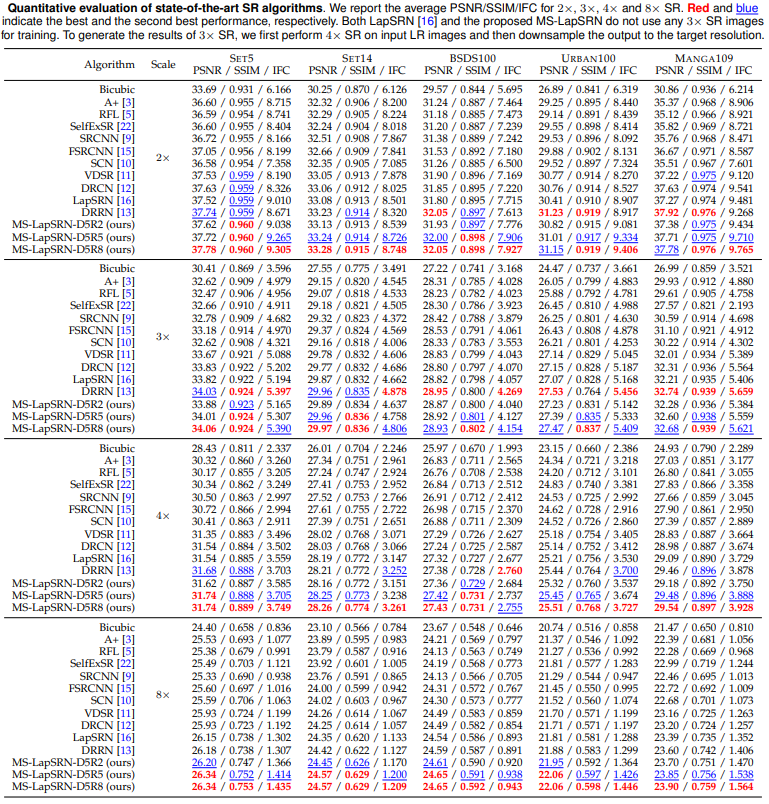
\includegraphics[width=\textwidth, keepaspectratio]{lapsr-sota-results.png}
        \caption{SOtA results up to now}
    \end{subfigure}
    \begin{subfigure}{0.49\textwidth}
        \centering
        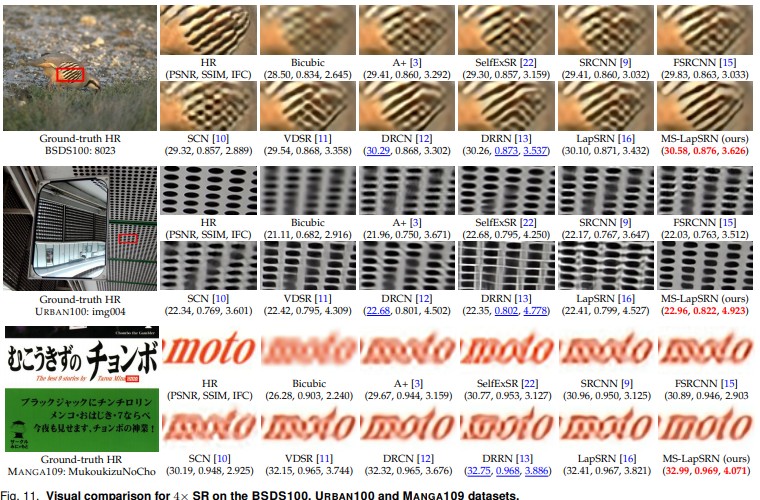
\includegraphics[width=\textwidth, keepaspectratio]{lapsr-result-urban-dataset.png}
        \caption{Qualitative results of MS-LapSRN.}
    \end{subfigure}
    \begin{subfigure}{0.49\textwidth}
        \centering
        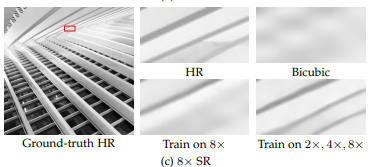
\includegraphics[width=\textwidth, keepaspectratio]{lapsr-multiscale-results.png}
        \caption{Multi-scale results of MS-LapSRN}
    \end{subfigure}
    \caption{Quantitative and qualitative results of MS-LapSRN}\label{lapsr:qq-results}
\end{figure}

Fro the quantitative and qualitative results [\Cref{lapsr:qq-results}] we can see that overall LapSRN performs better than state-of-the-art network, indeed it is able to reconstruct finer details thanks to the multi-scale training as we can see in the figure.